\documentclass[a4paper]{article}
\usepackage[a4paper,hmargin={3cm,2.5cm},vmargin={2.5cm,2.5cm}]{geometry}

\usepackage{tikz}
\usetikzlibrary{calc}

\usepackage{fancyhdr}
\pagestyle{fancy}
\lhead{}
\rhead{\textcolor{red}{Mini Project Title}}
\lfoot{Department of Computer Engineering}

\usepackage{lipsum}

\usepackage{multicol}

\usepackage{ragged2e}

\usepackage{xcolor}

\usepackage{enumitem}

\usepackage{caption}
\usepackage{subcaption}

\usepackage{listings}
\definecolor{mygreen}{rgb}{0,0.6,0}
\definecolor{mygray}{rgb}{0.5,0.5,0.5}
\definecolor{mymauve}{rgb}{0.58,0,0.82}

\lstset{
    backgroundcolor=\color{white},      % choose the background color; you must add \usepackage{color} or \usepackage{xcolor}; should come as last argument
    language=Python,                    % the language of the code
    basicstyle=\footnotesize\ttfamily,  % the size of the fonts that are used for the code
    breakatwhitespace=false,            % sets if automatic breaks should only happen at whitespace
    breaklines=true,                    % sets automatic line breaking
    captionpos=b,                       % sets the caption-position to bottom
    commentstyle=\color{mygreen},       % comment style
    deletekeywords={...},               % if you want to delete keywords from the given language
    escapeinside={\%*}{*)},             % if you want to add LaTeX within your code
    extendedchars=true,                 % lets you use non-ASCII characters; for 8-bits encodings only, does not work with UTF-8
    firstnumber=1,                      % start line enumeration with line 1
    numbers=left,                       % where to put the line-numbers; possible values are (none, left, right)
    numberstyle=\tiny\color{mygray},    % the style that is used for the line-numbers
    numbersep=7pt,                      % how far the line-numbers are from the code
	frame=single,                       % code snippet frame, t-> top, b->bottom, l->left, r->right, single-> all around
	tabsize=4,                          % tab = (tabsize) * space
    columns=flexible,                   % two options, fixed or flexible
    keepspaces=true,                    % keeps spaces in text, useful for keeping indentation of code (possibly needs columns=flexible)
    morekeywords={*,...},               % if you want to add more keywords to the set
    rulecolor=\color{black},            % if not set, the frame-color may be changed on line-breaks within not-black text (e.g. comments (green here))
	showspaces=false,                   % show spaces everywhere adding particular underscores; it overrides 'showstringspaces'
    showstringspaces=false,             % underline spaces within strings only
    showtabs=false,                     % show tabs within strings adding particular underscores
    stepnumber=1,                       % the step between two line-numbers. If it's 1, each line will be numbered
    stringstyle=\color{mymauve},        % string literal style
    title=\small\lstname,                     % show the filename of files included with \lstinputlisting; also try caption instead of title
	% keepspaces,
	keywordstyle=\color{blue}           % keyword style    
}

\usepackage{hyperref}

\begin{document}
\begin{titlepage}
    \begin{tikzpicture}[overlay,remember picture]
        \draw[line width=4pt]
        ($ (current page.north west) + (1cm,-1cm) $)
        rectangle
        ($ (current page.south east) + (-1cm,1cm) $);
        \draw[line width=1.5pt]
        ($ (current page.north west) + (1.2cm,-1.2cm) $)
        rectangle
        ($ (current page.south east) + (-1.2cm,1.2cm) $);
    \end{tikzpicture}

    \begin{center}

        \textup{\large  \textbf{INDIAN INSTITUTE OF ENGINEERING}\\\textbf{SCIENCE AND TECHNOLOGY, SHIBPUR}}\\ Howrah, West Bengal, India - 711103\\[0.5cm]\textbf{\large DEPARTMENT OF COMPUTER SCIENCE}\\\textbf{\large AND TECHNOLOGY}

        %---------------------------------Figure------------------------------
        \begin{center}
            \begin{figure}[h]   %h means here other options t , b, p, etc.
                \centering
                
\includegraphics[width=0.3\linewidth]{Pictures/IIESTS Logo.png}
            \end{figure}
        \end{center}

        %----------------------------

        \textup{\large A MINI-PROJECT REPORT SUBMITTED IN PARTIAL FULFILLMENT OF THE REQUIREMENTS\\[0.4cm]ON}\\[0.4cm]

        \begin{LARGE}
            {\textbf {\textcolor{red}{"MINI PROJECT TITLE"}}}
        \end{LARGE}\\[1cm]

        \textit{SUBMITTED BY}\\[0.3cm]
        \begin{large}
            \textbf{Abhinaba Chowdhury (510519007)}\\[0.1cm]
            \textbf{Abhiroop Mukherjee (510510109)}\\[0.1cm]
            \textbf{Debarghya Dey (510519087)}\\[0.1cm]
            \textbf{Jyotiprakash Roy (510519016)}\\[0.1cm]
            \textbf{Shrutanten (510519048)}\\[1cm]
        \end{large}

        \textit{UNDER THE GUIDANCE OF}\\[0.5cm]
        \begin{large}
            \textbf{DR. SAMIT BISWAS}\\[0.3cm]
        \end{large}

        \textbf{(Academic Year: 2020-2021)}
    \end{center}
\end{titlepage}
%================begin of certificate page======================

\begin{titlepage}
    \begin{tikzpicture}[overlay,remember picture]
        \draw[line width=4pt]
        ($ (current page.north west) + (1cm,-1cm) $)
        rectangle
        ($ (current page.south east) + (-1cm,1cm) $);
        \draw[line width=1.5pt]
        ($ (current page.north west) + (1.2cm,-1.2cm) $)
        rectangle
        ($ (current page.south east) + (-1.2cm,1.2cm) $);
    \end{tikzpicture}

    \begin{center}
        \textup{\large  \textbf{INDIAN INSTITUTE OF ENGINEERING}\\\textbf{SCIENCE AND TECHNOLOGY, SHIBPUR}}\\ Howrah, West Bengal, India - 711103\\[0.5cm]\textbf{\large DEPARTMENT OF COMPUTER SCIENCE}\\\textbf{\large AND TECHNOLOGY}

        %---------------------------------Figure------------------------------
        \begin{center}
            \begin{figure}[h]   %h means here other options t , b, p, etc.
                \centering
                
\includegraphics[width=0.3\linewidth]{Pictures/IIESTS Logo.png}
            \end{figure}
        \end{center}

        %----------------------------


        \begin{LARGE}
            \textbf{\textit {Certificate}}
        \end{LARGE}\\[1.2cm]
    \end{center}

    It is certified hereby that this report, titled *whatever the title is*, and all the attached
    documents herewith are authentic records of Abhinaba Chowdhury (510519007),\\Abhiroop Mukherjee (510510109), Debarghya Dey (510519087),
    Jyotiprakash Roy \\(510519016), and Shrutanten (510519048) from the Prestigious Department of \\Computer Science And Technology
    of the Distinguished and Respected IIEST Shibpur under my guidance.

    The works of these students are satisfies all the requirements for which it is submitted.
    To the extent of my knowledge, it has not been submitted to any different institutions for
    the awards of degree/diploma.

    \vspace{5cm}
    \begin{multicols}{2}
        \begin{center}
            \textbf{Dr. Samit Biswas\\Asst. Professor}\hspace{5cm}
        \end{center}
        \begin{center}
            \textbf{Dr. Sekhar Mandal\\Head Of Department}
        \end{center}
        \vspace{0.5cm}
    \end{multicols}
    \vfill
\end{titlepage}
%================end of title page======================

%----------------------ACKNOWLEDGEMENT---------------------------
\pagebreak
\newpage

\begin{titlepage}
    \begin{center}
        {\Large{\bf{\textit{ACKNOWLEDGEMENT}}\\[2cm]}}
    \end{center}


    \paragraph{\normalfont\textit{\indent We, as the students of IIEST, consider ourselves honoured to be working with Dr. Samit Biswas.
            The success of this project would not have been possible without his useful insights,
            appropriate guidance and necessary criticism.}}
    \paragraph{\normalfont\textit{\indent We would pass our token of token of gratitude to the Department of Computer Science And Technoogy as well for providing
            us with the opportunity to be able to tackle real world problems while improving
            our problem solving ability and thinking capacity by organising this project. We all have
            learnt quite a handful of new skills and are eager to use them henceforth as well.}}

    \begin{flushleft}
        \textit{Abhinaba Chowdhury (510519007)\\
            Abhiroop Mukherjee (510510109)\\
            Debarghya Dey (510519087)\\
            Jyotiprakash Roy (510519016)\\
            Shrutanten (510519048)}

    \end{flushleft}
\end{titlepage}

\pagenumbering{roman}
\setcounter{page}{1}
\newpage
\setcounter{tocdepth}{2} % + subsections
\tableofcontents
\lfoot{IIEST, Shibpur}
\newpage

\pagenumbering{arabic}
\setcounter{page}{1}

%%%%%%%%% MAIN TEXT STARTS HERE %%%%%%%%%%
\section{INTRODUCTION}
\subsection{Motivation}
Coronaviruses are a group of related RNA viruses that cause diseases in mammals
and birds. In humans and birds, they cause respiratory tract infections that can
range from mild to lethal. Mild illnesses in humans include some cases of the
common cold (which is also caused by other viruses, predominantly rhinoviruses),
while more lethal varieties can cause SARS, MERS, and COVID-19.

With the increase in the spread of the dangerous and highly contagious \textbf{Novel Coronavirus}
and the underlying disease caused by it, \textbf{COVID-19},
it is a requirement now more than ever to follow the social distancing
norms set in place by the scientists and researchers.

But as we all know, India is a country with a not-so-small population,
so it is pretty understandable and obvious that the law enforcement will
not be able to actually enforce it on every single person. Therefore,
new means of automata in place of actual individuals is a no brainier.

That is where we come in.

\subsection{The Idea Behind The Project}
The idea behind the working of this software was simple. The software just needed
to be able to look at a live feed (or recorded footage) of a camera and know
which of the people present in the footage are actually following the social
distancing norms and which of them are not, and mark either one appropriately.
That is where out journey to build a social distance checker started.

\textcolor{red}{// will add more later probably lul}

\newpage

\section{PREREQUISITES}

\subsection{Outdoor Requirements}
It is important to mention here that this is not a portable software that can
be fed any footage and just be expected to work. There need to be some
calibration measures taken to actually get this software working:

\begin{itemize}
    \item Actually knowing the local social distancing norms
          \begin{itemize}
              \item The minimum distance set for social distancing by the local government
          \end{itemize}

    \item Finding a good position for the camera
          \begin{itemize}
              \item The footage needs to be taken from a high enough place
          \end{itemize}

    \item Knowing the required distance in pixels
          \begin{itemize}
              \item This will depend on the position and angle of the camera's view
          \end{itemize}
\end{itemize}

\subsection{Hardware and Software Requirements}
The tools used to build this software are platform independent. However,
there are a few requirements needed to be fulfilled to get the program
working. These are:

\begin{itemize}
    \item Software Requirements
          \begin{itemize}
              \item Python - 3.5 or above
              \item OpenCV-Python - version 2 or above
              \item YOLOv3 Configuration and Network Weights
              \item Numpy
          \end{itemize}

    \item Hardware Requirements
          \begin{itemize}
              \item A GPU is optional yet recommended to get the best performance
              \item If a GPU is not being used, the CPU need to be good enough
          \end{itemize}
\end{itemize}

\section{THE PROJECT}
\subsection{Software Used}
The softwares used to build this \textit{checker} are:

\subsubsection{An Integrated Development Environment (IDE)}
An integrated development environment (IDE) is a software application that
provides comprehensive facilities to computer programmers for software
development. An IDE normally consists of at least a source code editor, build
automation tools and a debugger. Some IDEs contain the necessary compiler,
interpreter, or both; others, do not.

We used PyCharm as our IDE, as it was easy to set up and code

\textcolor{green}{wikipedia reference}PyCharm is an integrated development environment (IDE) used in computer programming, specifically for the Python language. It is developed by the Czech company JetBrains. It provides code analysis, a graphical debugger, an integrated unit tester, integration with version control systems (VCSes), and supports web development with Django as well as data science with Anaconda.

\subsubsection{Python}
Python is an interpreted, high-level and general-purpose programming language.
Python's design philosophy emphasizes code readability with its notable use of
significant whitespace. Its language constructs and object-oriented approach aim
to help programmers write clear, logical code for small and large-scale projects.

\paragraph{Why did we choose Python?}
\begin{enumerate}
    \item Python has an upper hand when it comes to software based on
          image recognition and object detection. Since it is the main
          objective of the project, choosing python was a given.Python has an upper hand when it comes to software based on
          image recognition and object detection. Since it is the main
          objective of the project, choosing python was a given.
    \item Python is unbeaten when it comes to Machine Learning. Python has
          support for myriad machine learning libraries, such as OpenCV, the
          one being used here.
    \item Python is comparatively easier to understand and learn. The syntax
          is clear and simple to read and write.
    \item And just our overall experience of using python for years.
\end{enumerate}

\subsubsection{Google Colab}
After working on the project for quite some time, we realized that we did
not have enough hardware resources at out disposal to actually make the
\textit{checker} work smoothly. So we decided on shifting to Google Colab.
Google colab is an online iPython development environment similar to
Jupyter Notebook. It uses CUDA acceleration to speed up processes, so we
switched to it rather than continuing development

\subsubsection{LaTeX}
LaTeX was used to write this report. LaTeX is a software system for document
preparation. When writing, the writer uses plain text as opposed to the formatted
text found in "What You See Is What You Get" word processors like Microsoft Word
or LibreOffice Writer.

\subsection{The Program}

\subsubsection{Outline}
The blueprint of this \textit{checker} that we thought of initially:

\begin{enumerate}
    \item Video Input
          \begin{itemize}[label={}]
              \item Need some way to handle video input coming through the camera feed
          \end{itemize}

    \item Processing
          \begin{itemize}[label={}]
              \item The input needs to be processed somehow
          \end{itemize}

    \item Detecting people
          \begin{itemize}[label={}]
              \item Need to identify people in the video feed
          \end{itemize}

    \item Measuring distance between each couple
          \begin{itemize}[label={}]
              \item Need to calculate the distance between every two persons
          \end{itemize}

    \item Mark the violations
          \begin{itemize}[label={}]
              \item Need to mark the ones that violate social distancing norms
          \end{itemize}
\end{enumerate}

\subsubsection{Proceedings}

How we proceeded with the outlines of the blueprint:

\begin{enumerate}
    \item Video Input
          \begin{itemize}[label={}]
              \item This was easier than we expected it to be. We just had to get our hands
                    on some recorded footage of somewhat populated areas. We refrained from using live
                    footage because:
                    \begin{itemize}
                        \item It is tough to get our hands on the light footage of a security camera or the equivalent.
                        \item If the checker worked on recorded footage, it would work on live footage as well.
                    \end{itemize}
                    \pagebreak
              \item The videos we ended up choosing:
                    \begin{figure}[h!]
                        \centering
                        \begin{subfigure}[b]{0.4\linewidth}
                            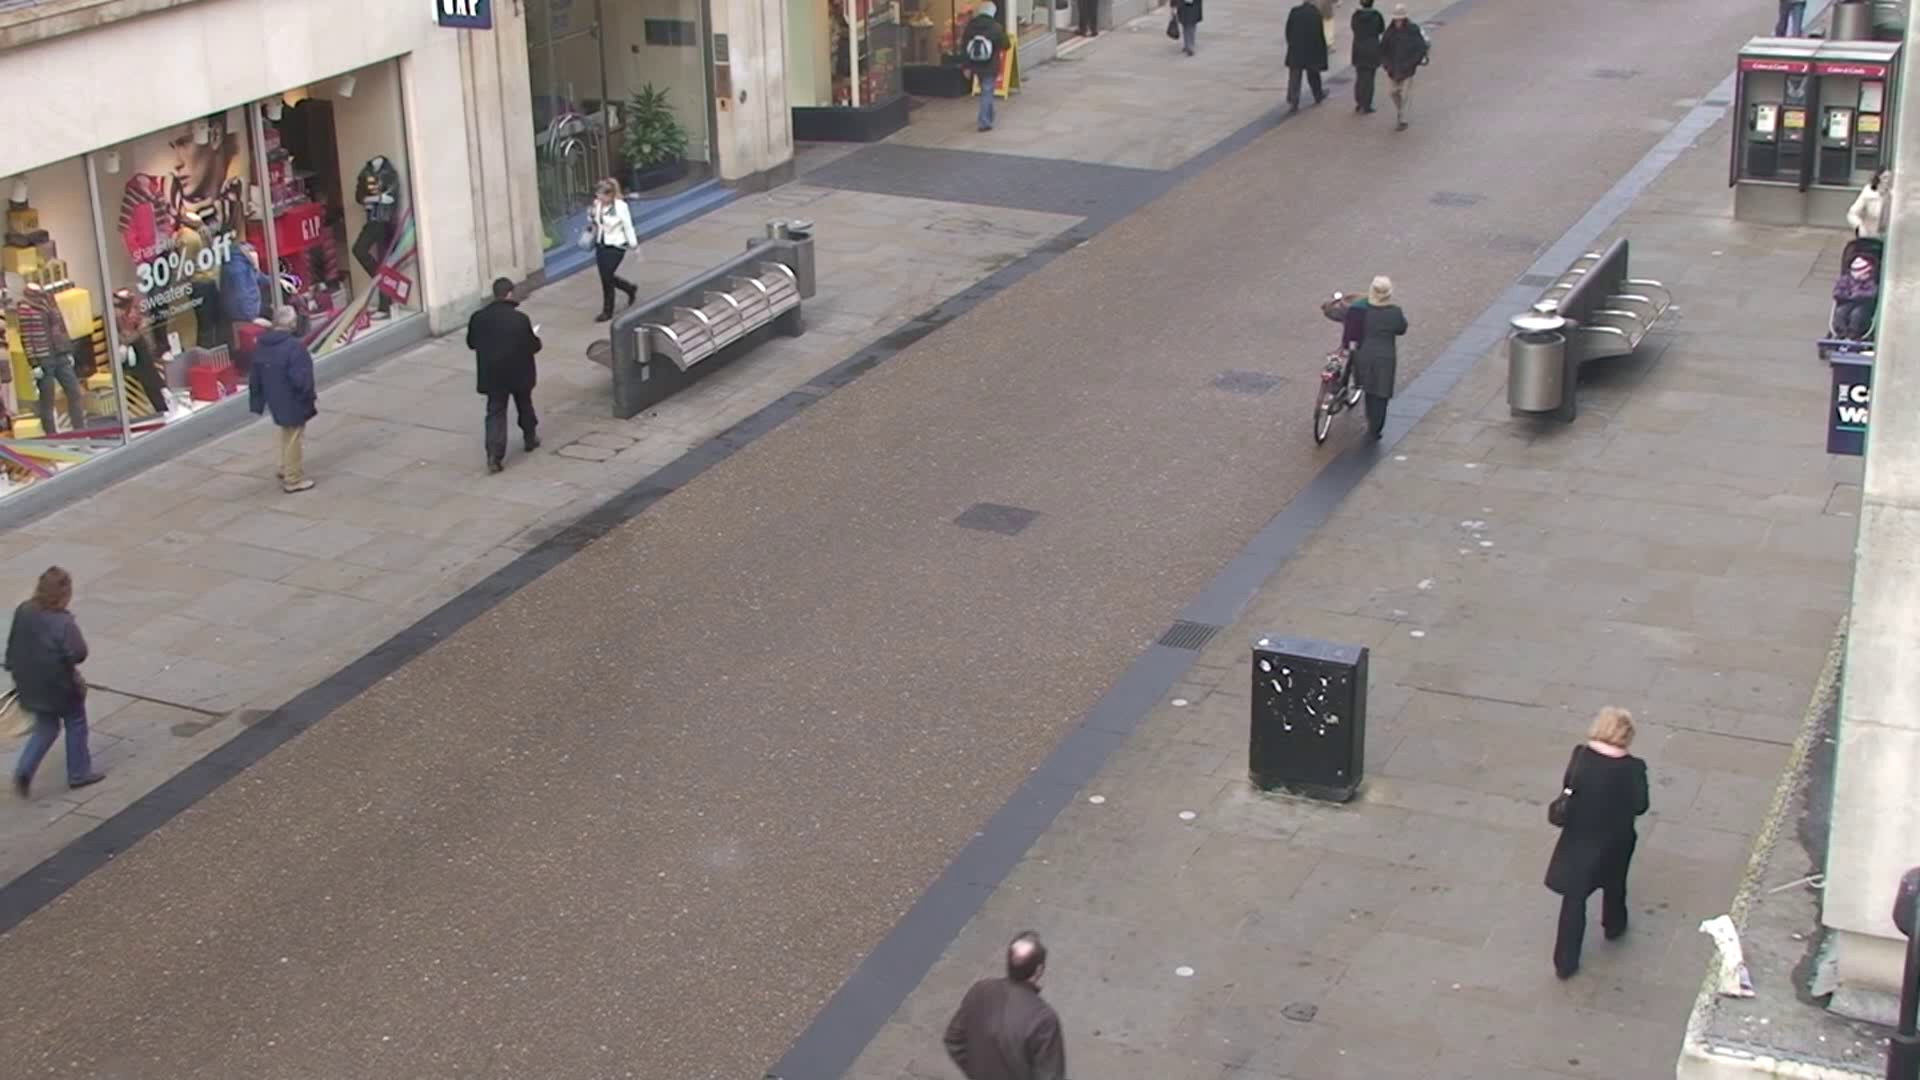
\includegraphics[width=\linewidth]{Pictures/pedestrian.jpg}
                            \caption{Pedestrian Video}
                        \end{subfigure}
                        \begin{subfigure}[b]{0.4\linewidth}
                            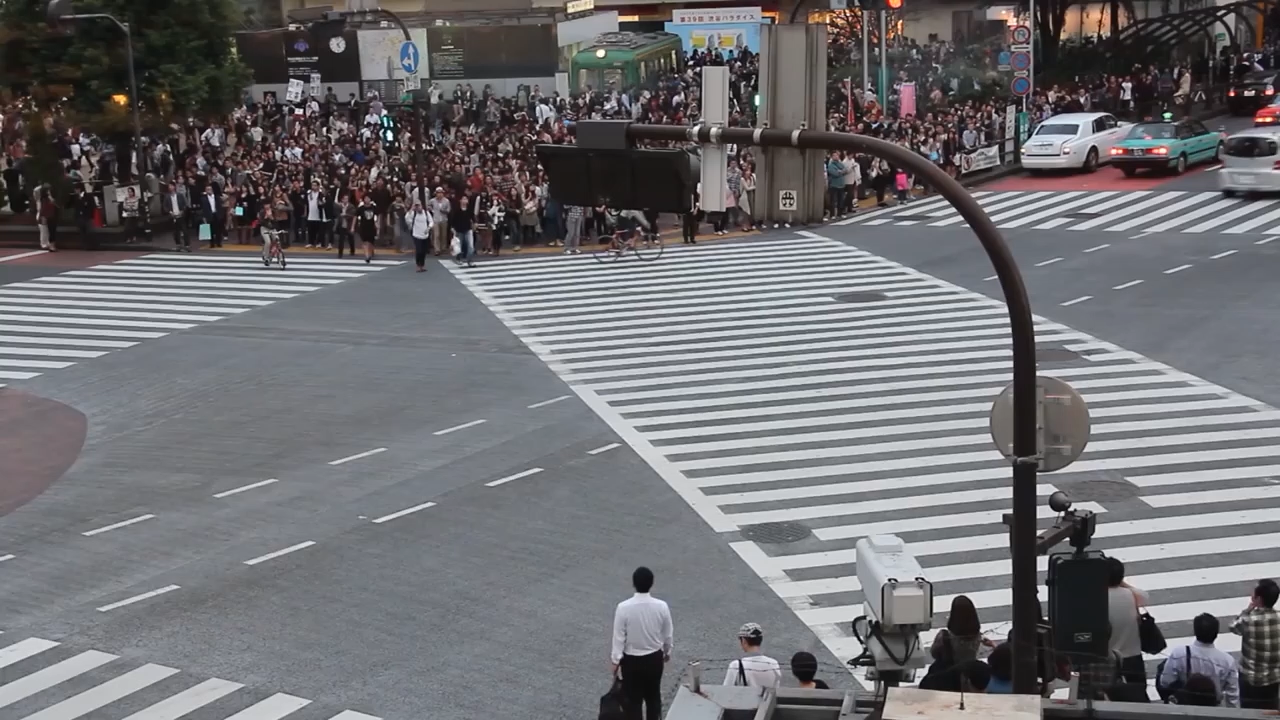
\includegraphics[width=\linewidth]{Pictures/shibuya.png}
                            \caption{Shibuya Video}
                        \end{subfigure}
                        \caption{Still Pictures from Sample Videos}
                        \label{fig1:stills}
                    \end{figure}
          \end{itemize}

    \item Processing
    \begin{itemize}[label={}]
        \item We used the OpenCV library for our video/image processing. It is a really handy library that can be used for image processing, object detection and many other purposes.
        \lstinputlisting[caption=A Sample Code To Count No. Of Frames in a Video, label=lst1:VideoFrames]{python scripts/total_frames.py}
    \end{itemize}
    
    \item Detecting People
          \begin{itemize}
              \item For this we decided to go with the You Only Look Once (YOLO) algorithm for object detection. The algorithm itself is discussed a bit later in the report.
              \item We did not train the object detection neural network model ourselves. We used the prebuilt model, trained by the Darknet team \textcolor{green}{https://pjreddie.com/darknet/yolo/} because of time constraints.
          \end{itemize}

    \item Measuring distance between each couple
          \begin{itemize}
              \item This was undeniably the toughest part of the project and took the longest time. First we decided to go with measuring the distance between the centroids of every two detections. But that may not work in every condition since it depends on the placement of camera and the view angle from the ground and perpendicular to the ground.
              \item A conversion of the 3-dimensional footage being fed to the algorithm to 2-dimensions was more than necessary to get the top view of every frame to avoid the \textit{viewing angle problem}.
              \item Enter \textbf{Bird's Eye View (BEV)}. This is what we called the top view of every frame. This was made possible by OpenCV's \textcolor{brown}{getPerspectiveTransform()} and \textcolor{brown}{warpPerspective()} functions.
                    \lstinputlisting[caption=Function Bird's Eye Perspective Transformation Matrix, label=lst2:BirdsEyePerspective]{python scripts/birds_eye_perspective.py}
              \item \textcolor{green}{\href{https://cseweb.ucsd.edu/classes/wi07/cse252a/homography_estimation/homography_estimation.pdf}{homography estimation pdf}} This piece of code essentially calculates what is called a \textit{transformation matrix}  for the supplied image (frame) which can then be used to get the centroids of the points as seen from a vertical position directly above the center of the rectangle passed to the function.
                    \lstinputlisting[caption=Function which convert co-ordinates to it's bird's view co-ordinate, label=lst3:birdsEyeAllign]{python scripts/birds_eye_allignment.py}
              \item We used these functions to get a two dimensional view of every frame and calculate distance between every pair of detections (people).
          \end{itemize}

    \item Mark the violations
          \begin{itemize}[label={}]
              \item This was again a fairly easy step. We just needed the coordinates of the people in the \textit{violation zone} and make their detection rectangle red as opposed to green.
          \end{itemize}
\end{enumerate}

\subsection{The YOLO Algorithm}

\end{document}